\section{System Overview}
\label{sec:fdsp-tpcelec-overview}

The main difference between the \dword{dune} \dword{sp} detector and 
previous experiments or prototypes using the \dword{lar} technology is
that for the first time all the signal processing for the readout of the
\dword{apa}s' wires takes place inside the the \dword{lar}, in boards that 
are directly mounted on the \dword{apa}. Accordingly, the \dword{tpc} 
readout electronics are referred to as the \dword{ce}. The electronics are 
mounted inside the \dword{lar} to exploit the fact that charge carrier 
mobility in silicon is higher and that thermal fluctuations are lower 
at \dword{lar} temperature than at room temperature. For \dword{cmos} 
electronics, this results in substantially higher gain and lower noise 
at \dword{lar} temperature than at room temperature~\cite{larCMOS}.  
Mounting the front-end electronics on the \dword{apa} frames also minimizes 
the input capacitance, which also contributes to the noise reduction.  
Furthermore, placing the digitizing and multiplexing electronics inside 
the cryostat reduces the total number of penetrations into the cryostat 
and minimizes the number of cables coming out of the cryostat.  
As the full \dword{tpc} electronics chain for the \dword{spmod} includes 
many components on the warm side of the cryostat as well, the \dword{dune} 
consortium designated to organize development of this system is called 
the \dword{dune} \textit{Single-Phase \dword{tpc} Electronics} consortium. 
It is sometimes referred to as the \dword{ce} consortium for short.
In Section we start with a review of the considerations that
have lead to the proposed design for the \dword{dune} \dword{sp} detector,
followed by a discussion of how the detector specifications are derived
from the physics goals of the experiment. Later we demonstrate the 
validation of the design provided by the early data from the \dword{pdsp}
prototype. We also discuss how the lessons learned from the construction,
integration, installation, and commissioning of \dword{pdsp} have 
informed the design changes that we are planning for the \dword{dune}
\dword{sp} detector. In the rest of this Chapter we provide a detailed
description of all the \dword{ce} detector components in Section
\ref{sec:fdsp-tpcelec-design}, followed by discussions of the \dword{qa}
program and of the plans for production and assembly, and for integration,
installation and commissioning. Later, we discuss the interfaces with
detector components provided by other consortia and with Technical
Coordination and the Physics group. This Chapter concludes with a description
of the plans for addressing safety issues and risks during the
construction, installation, and operation of the detector, and with
a discussion of the organization of the \dword{ce} consortium,
including a timeline for the detector construction and an estimate
of the resources required.

%%%%%%%%%%%%%%%%%%%%%%%%%%%%%%%%%%%
\subsection{Introduction}
\label{sec:fdsp-tpcelec-overview-intro}

\fixme{The following assumes that in the executive summary chapter we have
one section that describes the signal formation in the TPC. That section
should be based on Bruce Baller's summary paper (arXiv:1703.0424), with
numbers tailored to the DUNE-SP case.}

In the \dword{dune} \dword{spmod} a \dword{mip} deposits on average between
\SI{20}{k}{e$^-$} and \SI{30}{k}{e$^-$} on each collection wire, assuming an electron field
of \SI{0.5}{kV/cm} and an electron lifetime of \SI{6}{ms}, as discussed in
Chapter~\ref{ch:sp-execsum}, and assuming full transparency during the 
electron transport through the grid plane and the two plane of induction
wires as discussed in Chapter~\ref{ch:fdsp-apa}. The highest of the two numbers 
is for \dwords{mip} close to the collection plane, and the smallest of the two
takes into account the charge recombination effects caused by impurities for 
tracks close to the cathode plane. The \dword{dune} \dword{sp} \dword{tpc} is 
a unit gain device where the electrical signal is produced by the drift of the
charges near the wires, differently from what happens in gaseous wire 
chambers where the electrical field is strong enough to provide additional
ionization and signal multiplication. The signal induced in the \dword{dune}
\dword{spmod} wires is bipolar on the induction wires, positive when the
electrons drift toward the wires, and negative when they drift away from
the wires. On the collection wires signals are mostly unipolar (positive).
The signal duration is of the order of microseconds, and tends to be narrower
for the collection plane due to the increase of the electrical field and
therefore of the electron velocities.

The noise level enabled by having the front-end electronics in the cold (roughly 
half as much noise at \dword{lar} temperature than at room temperature) greatly 
extends the reach of the \dword{dune} physics program. Decreasing the noise level 
allows measurement of smaller charge deposits, a source of risk mitigation in 
case the desired drift field cannot be reached or the electron lifetime in the 
detector is less than desired (due to the electronegative impurities in the 
detector). For example, given an electron lifetime of \SI{3}{ms} and an electron field
of \SI{0.25}{kV/cm} the charge deposited in the collection wires from a 
\dword{mip} close to the cathode plane is reduced to \SI{10}{k}{e$^-$}.
The exact requirement of the minimal \dword{snr} required for pattern
recognition depends on the tracking algorithms and on the signal processing.
Initial studies for \dword{dune} indicated that a minimal \dword{snr} of 9 
on both the collection and induction wires was necessary. The 
\dword{sbnd} experiment prefers a minimal \dword{snr} of 12 for the
collection wires and of 5 for the induction wires~\cite{bib:sbnddoc1921}, taking into account
the difference between the signal amplitude in the two cases and considering
also the gain coming from fitting the bipolar shape of the signal on the
collection wires. For the design of the signal processing hardware for the
wires of the \dword{dune} \dword{spmod} we are setting a specification of
a total noise of less than 1000 e$^-$ consistent with having a \dword{snr}
of at least 10 on the collection wires even in the pessimistic case 
where the electron lifetime and the electric field just meet the
required design values discussed in Chapter~\ref{ch:sp-hv}.

The goal is to keep the total noise level as low as possible. For example an 
increase in the \dword{snr} above 15 allows the observation of MeV scale photons, 
as recently demonstrated by \dword{argoneut}~\cite{Acciarri:2018myr}, enabling 
reconstruction of photons released during de-excitation of the nucleus and of part
of the energy transferred to final-state neutrons.
Decreasing the noise level also increases the reach of low-energy 
physics measurements like those associated with stellar core-collapse supernova 
burst neutrinos. Finally, a low noise level opens up the possibility of using 
$\mathrm{{}^{39}Ar}$ beta decays to calibrate the \dword{dune} \dword{spmod}.
Finally the noise level has also consequences on the bandwidth requirements
for the \dword{daq} system, that are discussed in Chapter~\ref{ch-spdaq}.

To retain maximum flexibility in optimizing reconstruction algorithms after 
the \dword{dune} data is collected, the \dword{spmod} electronics are designed 
to produce a digital record representing the waveform of the current produced 
by charge collection/induction on the anode wires.  Each anode wire signal is 
input to a charge sensitive amplifier, followed by a pulse shaping circuit and 
an \dword{adc}.  To minimize the number of cables and cryostat penetrations, 
the \dwords{adc} as well as the amplifier/shapers are located in the \dword{lar}, 
and digitized data from many wires merge onto a much smaller set of high speed 
serial links. The \dword{ce} signal processing is implemented in \dfirsts{asic}
using \dword{cmos} technology.  The \dword{ce} is continuously 
read out, resulting in a digitized \dword{adc} sample from each \dword{apa} 
channel (wire). The \dwords{asic} used for the readout of the \num{2560}
wires of each \dword{apa} are house on \dfirsts{femb}, that are connected to
\dwords{wib} located the outside of the cryostat via a \dword{ce} signal 
cable flange located at the \dword{ce} \fdth at the top of the cryostat.
From the \dwords{wib} the data is sent to the \dwords{daq} beckoned on
an optical fiber network as discussed in Chapter~\ref{ch:sp-daq}.

%%%%%%%%%%%%%%%%%%%%%%%%%%%%%%%%%%%
\subsection{Requirements}
\label{sec:fdsp-tpcelec-overview-requirements}

In addition to the noise requirement (less than \num{1000}\,$e^{-}$), several 
additional requirements determine most of the other important \dword{dune} \dword{spmod}
electronics specifications. Some of them, labeled as SP-PD in Table~\ref{tab:specs:SP-TPC}
are derived from the overall physics goals of the experiment. The rest, labeled
as SP-TPC, are engineering requirements derived from the design choices that
are discussed later in this Chapter.

%%\input{generated/req-longtable-SP-TPC}

\begin{itemize}
\item{The \dword{fe} peaking time must be in the range \numrange{1}{3}\,\si{\micro\second},
to match the time required for the drifting charges to travel from one plane of anode
wires to the next. The planes of anode wires are separated by \SI{4.75}{mm}
as discussed in Chapter~\ref{ch:fdsp-apa}, and the drift velocity for
the electrical fields considered for \dword{dune} is in the range
\SIrange{1.25}{1.5}{mm/$\mu$s}.}
\item{The system must have a linear response up to an impulse input of 
at least \num{500000}\,$e^{-}$.  This roughly corresponds to the largest 
ionization signals expected in events where multiple protons are produced 
in the primary event vertex, in particular, when the trajectories of one 
or more of those particles are parallel to the wire, causing the charge 
over a long path length to be collected within a short time.}
\item{The \dword{adc} sampling frequency must be \SI{{\sim}2}{MHz},
This value is chosen to match a \dword{fe} shaping time of \SI{1}{\micro\second} 
(approximate Nyquist condition) while minimizing the data rate.}
\item{The \dword{adc} must digitize the charge deposited on the wires 
with 12~bits of precision.  The lower end of the \dword{adc} dynamic 
range is driven by the requirement that the ADC digitization does not 
contribute to total electronics noise. The upper end of the \dword{adc} 
dynamic range is defined by the previous requirement for the signal 
saturation level. Combining these two requirements with the specification 
for the total electronics noise results in the need for 12~bits digitization.}
\item{The power dissipated by the electronics located in the \dword{lar} must
be less than \SI{50}{mW/channel}.  Lower power dissipation is desirable 
because the mass of the power cables scales with  power. Ongoing studies 
focus on whether the amount of power dissipated by the electronics 
should be minimized further because of potential complications from 
argon boiling; in principle, this should not be a problem because the 
\dword{ce} boxes housing the \dwords{femb} are designed to channel 
bubbles to the \dword{apa} frames.}
\item{All the components of the readout chain, including the \dword{adc}
and the bias voltage supplies, must not contribute significantly to
the overall noise of the readout chain. In the case of the \dword{adc}
this requirement depends on the gain of the \dword{fe} and
for each gain setting it translates into requirements on
the \dword{adc} parameters, including non-linearity and noise.}
\item{The fraction of non-functioning channels over the \dunelifetime
nominal life time of the \dword{dune} experiment should not
exceed 1\%. Studies are ongoing to quantify the effect of failures
in the \dword{tpc} and electronics, including
single wire failures, and failures of groups of
\num{16}, \num{64}, or \num{128} channels.}
\item{The \dword{fe} must have an adjustable baseline such that both the
bipolar signal from the induction wires and the mostly unipolar signal 
from the collection wires can be processed with a single amplifier.}
\item{The readout electronics for the \dword{apa} wires must be organized
in \dword{femb} containing 128 channels. This number is a sub-multiple
of the number of wires on an \dword{apa} and is also determined
by geometrical consideration on the number, size, and form
factor of the CR boards introduced in Section~\ref{sec:crboards}.}
\item{The data from the \dwords{femb} must be transmitted to the
\dwords{wib} on a maximum of 4 links per board, to minimize
the number of connections on the cryostat penetrations. This however 
requires data transmission at higher speeds and therefore larger power 
consumption inside the \dword{lar}. High data transmission speeds may 
also result in unacceptable bit error rates particularly for the 
\SI{\sim23.5}{m} links for the bottom \dword{apa}. A reduction of
the number of links per \dword{femb} to 2 should be investigated.}
\item{Each \dword{wib} must read-out four \dwords{femb}. This number
is a balance between the complexity of the boards, the mechanics
of the \dword{wiec} that houses the \dwords{wib}, and the 
required processing power in the \dword{fpga} inside the
\dword{wib} that is used to further serialize the data 
before transmission to the \dword{daq} back-end.}
\item{Each \dword{wib} must transmit data to the \dword{daq}
back-end on optical links at a speed of \SI{~10}{Gbps}. This speed 
is a compromise between the cost of optical transmitters and
receivers and the complexity of the readout fiber plant.}
\item{All the cables required to provide the low voltage power
and the control and readout for the \dwords{femb} mounted on
the bottom \dword{apa}, plus the bias voltage cables for
the same \dword{apa}, must fit inside two conduits with a
diameter of \SI{2.5}{in} that are inserted in the frame of
the \dword{apa}, as discussed in Section~\ref{sec:fdsp-apa-intfc}.}
\end{itemize}

%%%%%%%%%%%%%%%%%%%%%%%%%%%%%%%%%%%
\subsection{Design Considerations}
\label{sec:fdsp-tpcelec-overview-design}

The baseline design of the \dword{ce} detector components is
based on the specifications presented in the previous Section.
Each individual \dword{apa} has \num{2560} channels read out by \num{20} 
\dfirsts{femb}, with each \dshort{femb} enabling digitized wire readout 
from \num{128} channels. One cable bundle connects each \dshort{femb} to
the outside of the cryostat via a \dword{ce} signal cable flange located 
at the \dword{ce} \fdth at the top of the cryostat, where a single flange 
services each \dword{apa}, as shown in Figure~\ref{fig:connections}. 
Two \dword{ce} signal flanges are on each \fdth and together account for 
all electronics channels associated with a pair of \dword{apa}s (upper 
and lower, vertically arranged). Each cable bundle contains wires for 
low-voltage (\dword{lv}) power, high-speed data readout, and clock or 
digital-control signal distribution. Eight separate cables carry the 
\dword{tpc} wire bias voltages from the signal flange to the \dword{apa} 
wire bias boards, in addition to the bias voltages for the field cage 
termination electrodes and for the electron diverters. An additional 
flange on the top of each \fdth services the \dword{pds} cables associated 
with the \dword{apa} pair. Low voltage power supplies and bias voltage
power supplies are located on the top of the cryostat. 

\begin{dunefigure}
[Connections between the signal flanges and \dword{apa}]
{fig:connections}
{Connections between the signal flanges and \dword{apa}. The lower 
\dword{apa} shares the photon detector flange with the 
upper \dword{apa} but has a separate TPC readout flange. 
A \textit{\dword{ce} module} consists of all \dword{ce} 
associated with \num{128} channels of digitized readout.}
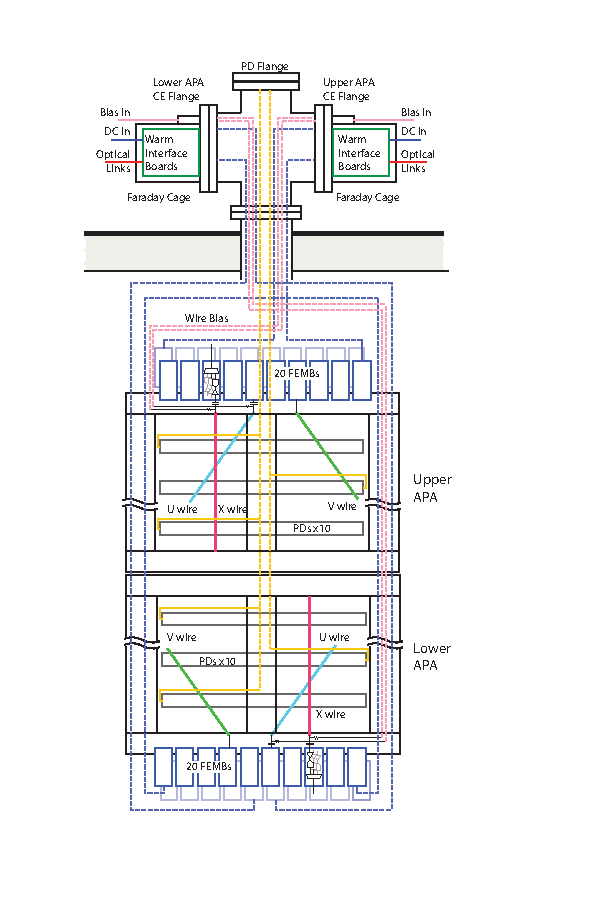
\includegraphics[width=0.7\textwidth]{sp-tpcelec-DUNE-FD-APA-readout-scheme-v1.pdf}
\end{dunefigure}

The components of the \dword{ce} system are the following:
\begin{itemize}
\item{\dwords{femb}, on which the \dwords{asic} are mounted, and 
which are installed on the \dword{apa}s;}
\item{cables for the data, clock, and control signals; \dword{lv} 
power; and wire bias voltages between the \dword{apa} and the 
signal flanges (cold cables);}
\item{signal flanges with a \dword{ce} \fdth to pass the data, clock, 
and control signals; \dword{lv} power; and \dword{apa} wire-bias 
voltages between the inside and outside of the cryostat; and 
the corresponding cryostat penetrations and spool pieces;}
\item{\dwords{wiec} mounted on the signal flanges and contain
the \dwords{wib} and \dwords{ptc} for further processing
and distribution of the signals entering and exiting the cryostat;}
\item{cables for \dword{lv} power and wire bias voltages between 
the signal flange and external power supplies (warm cables); and}
\item{\dword{lv} power supplies for the \dword{ce} and bias-voltage 
power supplies for the \dword{apa}s.}
\end{itemize}

\begin{dunetable}
[TPC electronics components and quantities for a single \dword{apa} of a \dword{spmod}.]
{llr}
{tab:elecNums}
{TPC electronics components and quantities for a single \dword{apa} of the DUNE \dword{spmod}.}
\textbf{Element} &\textbf{Quantity} & \textbf{Channels per element}\\ \toprowrule
Front-end mother board (\dword{femb}) & \num{20} per \dword{apa} & \num{128} \\ \colhline
FE \dword{asic} chip & \num{8} per \dword{femb} & \num{16} \\ \colhline
\dword{adc} \dword{asic} chip & \num{8} per \dword{femb} & \num{16} \\ \colhline
\dword{coldata} \dword{asic} chip & \num{2} per \dword{femb} & \num{64} \\ \colhline
Cold cable bundle & \num{1} per \dword{femb} & \num{128} \\ \colhline
Signal flange & \num{1} per \dword{apa} & \num{2560} \\ \colhline
\dword{ce} \fdth & \num{1} per \dword{apa} pair & \num{2560} \\ \colhline
Warm interface board (\dword{wib}) & \num{5} per \dword{apa} & \num{512} \\ \colhline
Warm interface electronics crate (\dword{wiec}) & \num{1} per \dword{apa} & \num{2560} \\ \colhline
Power and timing card (\dword{ptc}) & \num{1} per \dword{apa} & \num{2560} \\ \colhline
\end{dunetable}

The baseline design for the \dword{spmod} TPC electronics calls for three 
types of \dwords{asic} inside  the \dword{lar}:
\begin{itemize}
\item{a \num{16}-channel \dword{fe} \dword{asic} for amplification 
and pulse shaping (referred to as \dword{larasic});}
\item{a \num{16}-channel \num{12}-bit \dword{adc} \dword{asic} 
operating at \SI{{\sim}2}{MHz}; and}
\item{a \num{64}-channel control and communications \dword{asic} 
(referred to as \dword{coldata}).}
\end{itemize}

TALK ABOUT PROTODUNE HERE. THE FOLLOWING TEXT SHOULD BE MOVED LATER.

The \dword{fe} \dword{asic} has been prototyped and is close to meeting 
requirements (discussed in Section~\ref{sec:fdsp-tpcelec-overview-scope}). 
Another prototype to address issues in the version deployed in \dword{pdsp} 
will be developed in 2019. Key portions of \dword{coldata} have been
prototyped and meet requirements, and a first complete prototype of
\dword{coldata} will be submitted for fabrication in March 2019.
\dword{asic} (also called the \dword{coldata} \dword{asic}) have been prototyped and meet requirements.  However, we have determined that the BNL-designed P1-\dword{adc} \dword{asic} now being used in \dword{pdsp} does not meet requirements, and accordingly, its development has been terminated.  A new \dword{adc} \dword{asic} (also called the cold \dword{adc} \dword{asic}) is being developed by an LBNL-\fnal-BNL collaboration; first prototypes should be ready in February 2019.  The first full prototype of the controls and communication \dword{asic} should also be available for testing in June 2019.

To maximize the probability of quickly developing a complete design for cold TPC \dword{fe} electronics, an alternative solution is also being investigated: a single \num{64}-channel \dword{asic} that will consolidate all three functions listed above.  This design is being done at SLAC, and the first prototypes will be tested in February 2019.  An \dword{adc} solution in the form of a commercial, off-the-shelf (COTS) option serves as an additional backup option and has already been tested; this option will be explored further if the other two \dword{adc} solutions being considered do not meet the requirements for \dword{dune}.

While the higher charge carrier mobility at \dword{lar} temperature than at room temperature is central to improving the performance of \dword{ce}, it also leads to the \textit{hot carrier effect}.  In n-type \dword{cmos} transistors, the carriers (electrons) can acquire enough kinetic energy to ionize silicon in the active channel.  This charge can become trapped and lead to effects (including threshold shifts) similar to those caused by radiation damage.  This effect can cause MOS circuits to age much more quickly at \dword{lar} temperature than at room temperature, reducing performance and potentially causing failure.  To mitigate this effect, the maximum \efield in transistor channels must be lower than the field that can be reliably used at room temperature.  This is accomplished by using transistors fabricated longer than is typical and operated at reduced bias voltage.  Any commercial circuits used in the \dword{lar} must be carefully tested to ensure they will perform well for the expected \num{20}-year lifetime of \dword{dune}; reliability studies for front-end electronics designs in consideration are discussed in Section~\ref{sec:fdsp-tpcelec-qa-reliability}.

A series of tests are planned to demonstrate that the \dword{ce} system design will meet \dword{dune} requirements. These include two system tests: one using the \dword{pdsp} \textit{cold box} at CERN and one using a new small \dword{lartpc} at \fnal. The latter will also accommodate one half-length \dword{dune} \dword{pd} and will provide a low-noise environment that will allow detailed comparisons of the performance of the new \dwords{asic}. It will also enable the study of interactions between the \dword{tpc} readout and other systems, including the \dword{pd} readout and the \dword{hv} distribution. These test facilities are discussed in more detail in Section~\ref{sec:fdsp-tpcelec-qa-facilities}. A second period of data taking is also planned for the \dword{pdsp} detector, with final \dword{apa}s including the final \dwords{asic} and \dwords{femb} replacing the current prototypes. This second run of \dword{pdsp} is planned for 2021-2022.

\fixme{Update on second ProtoDUNE run?  Also discuss more what can be done with current ProtoDUNE run}

%%%%%%%%%%%%%%%%%%%%%%%%%%%%%%%%%%%
\subsection{ProtoDUNE-SP Results}
\label{sec:fdsp-tpcelec-overview-pdune}

\fixme{A discussion of ProtoDUNE studies that the CE consortium needs should be discussed at an upcoming CE consortium meeting; this discussion and subsequent plans will inform the updating of this section for the second draft}

The Single Phase \dword{protodune}-\dword{sp} detector, described in Chapter~\ref{ch:sp-execsum}, is a 700~ton fiducial volume \dword{lartpc} with 15,360 sense wires that are read out by the \dword{ce} system described in Section~\ref{sec:fdsp-tpcelec-qa-facilities-pdune}. The system was deployed in a beam line of the CERN Neutrino Platform in 2018 and continues to take cosmic event data into 2019. The goal of the \dword{protodune}-\dword{sp} \dword{tpc} readout was to validate the concept and the design of the integrated \dword{apa}+\dword{ce} readout and measure the performance of the \dword{ce} system with components as close as possible to the final \dword{dune} \dword{tpc} readout.

Each of the six \dword{protodune}-\dword{sp} \dword{apa}+\dword{ce} readout units consists of 2,560 sense wires, of which 960 are \SI{6}{m} long collection wires and 1,600 are \SI{7.4}{m} long induction wires. Each one was tested in a full scale cold box in cold gaseous Nitrogen (GN2) with a complete \dword{ce} readout system identical to the one on the detector before installation in the cryostat. Figure~\ref{fig:apa2-cycle} shows the \dword{enc}, which is the charge in electrons that would have to arrive at the sense wires to generate a signal with the \rms measured by the front end electronics as a function of cold cycle time. At a stable temperature of \SI{160}{K} the \dword{enc} for all three wire planes is less than 500~e$^-$.

\begin{dunefigure}
[\dword{pdsp} APA2 noise levels measured in GN2 at CERN Cold Box]
{fig:apa2-cycle}
{Left Y-axis: ENC (in electrons) for U, V, and X (red, blue, and green curves) sense wire planes as a function of time (hours) for the APA2 cold cycle in GN2 in the CERN Cold Box; right Y-axis: temperature (orange curve) measured at the level of the front-end electronics.}
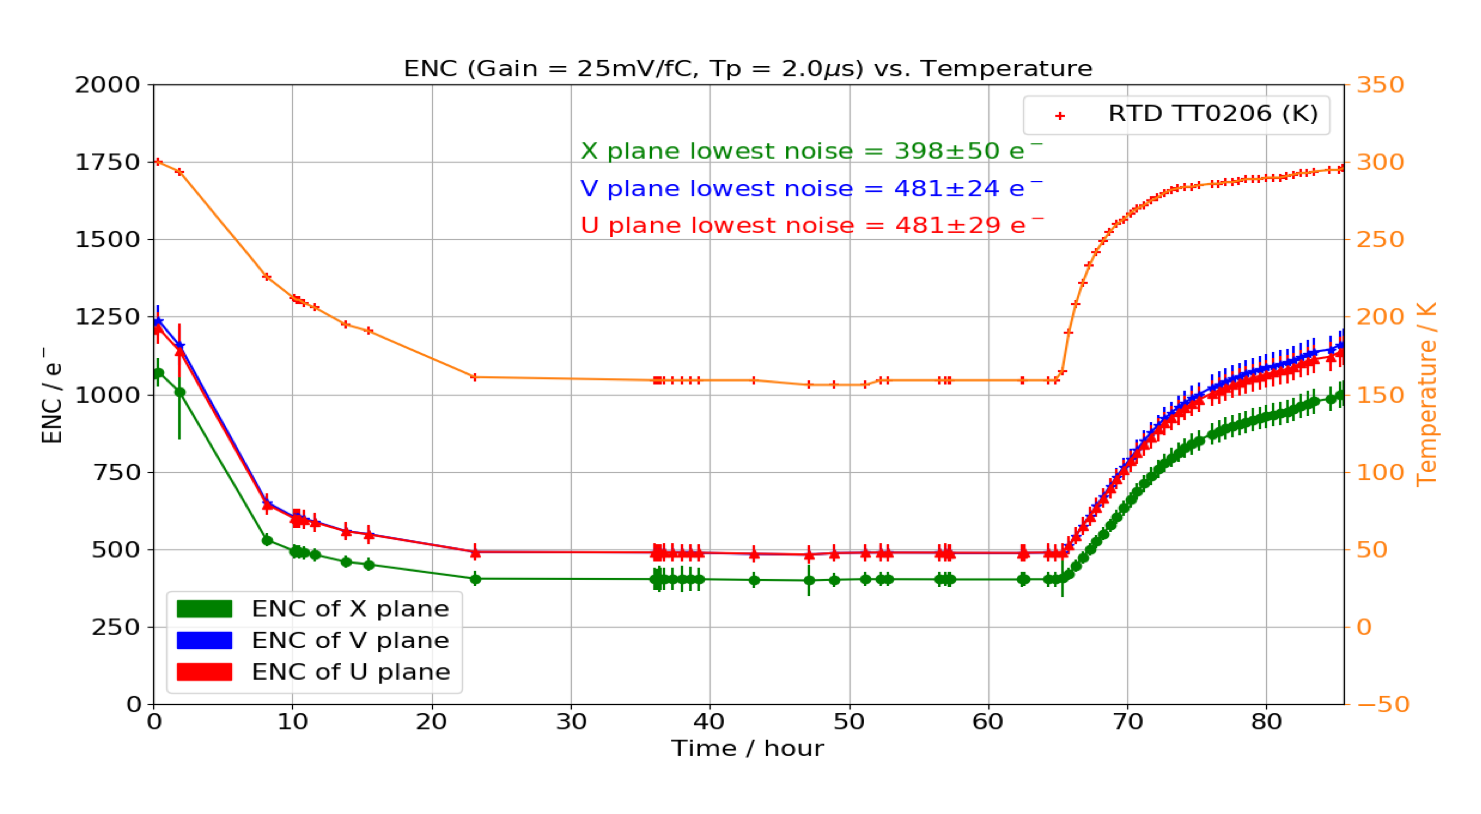
\includegraphics[width=1.0\linewidth]{sp-tpcelec-apa2.png}
\end{dunefigure}

After the cryostat was filled with \dword{lar} and the drift and wire bias HV were set to nominal (defined in Chapter~\ref{ch:sp-execsum}), 99.7\% of the \dword{tpc} readout channels were alive. The following channels were expected to be unresponsive to charge deposited on the wires:
\begin{itemize}
\item Four electronics channels, suggesting a dead channel in the electronics, all on collection wires on three different \dwords{apa};
\item $\sim$35 channels measured with  consistent with no capacitive load on the \dword{fe} electronics, suggesting an open connection somewhere in front of the \dword{ce} system, scattered randomly throughout the detector and on all wire planes.
\end{itemize}
With the detector in nominal operating conditions, the \dword{enc} was approximately 550~e$^-$ on the collection wires and approximately 750~e$^-$ averaged over all operational channels. Figure~\ref{fig:apa3-noise} shows the \dword{enc} in electrons for all channels of one of the \dword{apa}+\dword{ce} readout units. The collection channels with \dword{enc}$>$1500~e$^-$ are caused by an artifact in the generation of cold \dword{adc} \dword{asic} used in \dword{protodune}-\dword{sp}. The channels in all three planes with \dword{enc}$<$300~e$^-$ have an open connection somewhere in front of the \dword{ce} system.

\begin{dunefigure}
[TPC noise levels measured at \dword{pdsp} after \lar fill]
{fig:apa3-noise}
{ENC (in electrons) for all U, V, and X (red, blue, and green curves) sense wire planes for one ProtoDUNE APA with the detector in nominal operating conditions.}
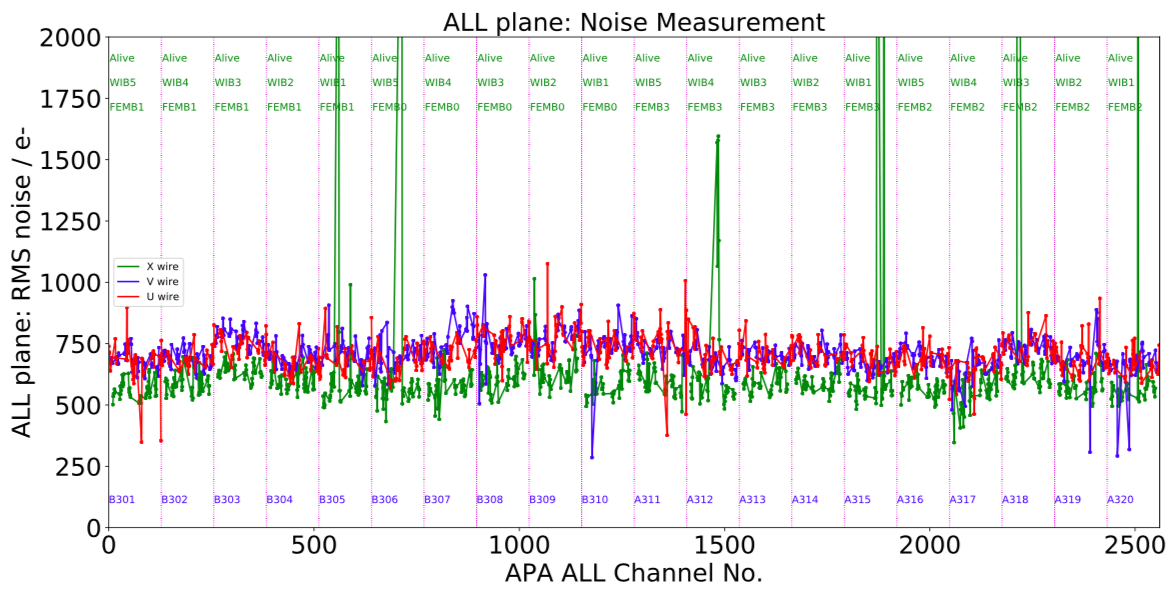
\includegraphics[width=1.0\linewidth]{sp-tpcelec-apa3-enc.png}
\end{dunefigure}

The overall performance of the \dword{ce} system in \dword{protodune}-\dword{sp} satisfies the \dword{dune} single phase \dword{fd} \dword{ce} system requirements listed in Section~\ref{sec:fdsp-tpcelec-overview-scope}. The overall system architecture, described in Section~\ref{sec:fdsp-tpcelec-overview-design}, will remain the same for the \dword{dune} \dword{ce}. However, several improvements and updates to the \dword{ce} system design were motivated by the results of the testing and commissioning of, and the data-taking with, the \dword{protodune}-\dword{sp} electronics. They will be discussed in this Section.

\fixme{Should show noise levels for all APAs in Figure~\ref{fig:apa3-noise}, not just APA 3...}
%%%%%%%%%%%%%%%%%%%%%%%%%%%%%%%%%%%
\subsection{ProtoDUNE-SP Lessons Learned}
\label{sec:fdsp-tpcelec-overview-lessonslearned}

\fixme{Add lessons learned here}
